%$Header: /usr/local/ollincvs/Codes/OllinSphere-BiB/doc/usermanual.tex,v 1.50 2024/06/10 18:24:14 malcubi Exp $

%-----------------------------------------------------------------------
%
% filename = usermanual.tex
% 
%-----------------------------------------------------------------------

\documentclass[12pt]{article}

% Load packages for symbols and figures.

\usepackage{latexsym}
\usepackage{epsfig}
\usepackage{amssymb}
\usepackage{tikz}
\usetikzlibrary{shapes}

% Page settings.

\setlength{\textwidth}{170mm}
\setlength{\oddsidemargin}{-5mm}
\setlength{\evensidemargin}{-5mm}


%%%%%%%%%%%%%%%%%%%%%%%%%%
%%%   BEGIN DOCUMENT   %%%
%%%%%%%%%%%%%%%%%%%%%%%%%%

\begin{document}

% Reference equations with section number.

\renewcommand{\theequation}{\thesection.\arabic{equation}}

\parindent 0mm


%%%%%%%%%%%%%%%%%
%%%   TITLE   %%%
%%%%%%%%%%%%%%%%%

\title{Code \texttt{OllinSphere-BiB} \\ User's manual}

\author{Miguel Alcubierre \\
Instituto de Ciencias Nucleares, UNAM \\
malcubi@nucleares.unam.mx}

\date{June, 2018}

\maketitle

\tableofcontents


%%%%%%%%%%%%%%%%%%%%%%%%
%%%   INTRODUCTION   %%%
%%%%%%%%%%%%%%%%%%%%%%%%

\pagebreak

\section{Introduction}

The program \texttt{OllinSphere-BiB} solves the Einstein evolution
equations in spherical symmetry, using a curvilinear version of the
BSSN formulation for the 3+1 evolution equations, with different types
of matter and different gauge conditions. \\

The main difference of this version of the code with respect to
previous ones is the fact that it uses box-in-box mesh refinement
(hence the BiB part of the name), and is parallelized with MPI
(Message Passing Interface). \\

Note: This manual is perpetually incomplete since I keep adding new
things to the code. Still, it should give you a good idea of the
basics. If you find something wrong please let me know! \\


%%%%%%%%%%%%%%%%%%%%
%%%   DOWNLOAD   %%%
%%%%%%%%%%%%%%%%%%%%

\section{Downloading the code}

If you are reading this it means you probably already downloaded the
code.  But if for some reason you need to download it here is how. \\

\subsection{From CVS}

The easiest way to obtain the code is to download it from the CVS
server of the Ollin group (unfortunately, since CVS is rather old, now
this only works from within my own Institute's network). In order to
obtain a username and password for this sever you need to contact
Miguel Alcubierre (malcubi@nucleares.unam.mx). Once you have a
username and password you first need to log into the repository by
typing at the terminal: \\

\texttt{\footnotesize cvs -d
  :pserver:username@dulcinea.nucleares.unam.mx:/usr/local/ollincvs
  login} \\

where you should change the word ``username'' for your personal
username! You then need to type your password.  After this you must
download the code by typing: \\

\texttt{\footnotesize cvs -d
  :pserver:username@dulcinea.nucleares.unam.mx:/usr/local/ollincvs co
  Codes/OllinSphere-BiB} \\

This will create a directory \texttt{Codes} and inside it directory
\texttt{OllinSphere-BiB}. This is the main directory for the code.

\subsection{From GIT}

Another way to dowload the code is from the public GIT repository.
This is in fact easier than CVS: \\

\texttt{\footnotesize git clone https://github.com/malcubi/OllinSphere-BiB} \\

Once you hacve the code, you can get updated versions by just doing
``git pull'' inside the code main directory.


%%%%%%%%%%%%%%%%%%%%%%%
%%%   DIRECTORIES   %%%
%%%%%%%%%%%%%%%%%%%%%%%

\section{Directory structure}

The main directory for the code is \texttt{OllinSphere-BiB}.  There are
several sub-directories inside this main directory:

\begin{list}{}{
\setlength{\leftmargin}{40mm}
\setlength{\labelsep}{10mm}
\setlength{\labelwidth}{25mm}}

\item[\texttt{CVS}] Contains information about the CVS root and server (see
Sec.~\ref{sec:editing}).

\item[\texttt{doc}] Contains the tex and pdf files for this user's
  manual.

\item[\texttt{exe}] This directory is created at compile time and
  contains the executable file.  It also contains a copy of the
  parameter files found in directory \texttt{par} (see below).

\item[\texttt{fakempi}] Contains fake MPI routines so that the
  compiler won't complain if MPI is not installed.

\item[\texttt{gnuplot}] Contains a couple of simple gnuplot macros for
  visualization.

\item[\texttt{objs}] This directory is created at compile time and
  contains all the object and module files.

\item[\texttt{ollingraph}] Contains the visualization package
  ``ollingraph'' for convenient ``quick and dirty'' visualization (see
  Section~\ref{sec:ollingraph} below).

\item[\texttt{par}] Contains examples of parameter files (see
Section~\ref{sec:parfiles} below).

\item[\texttt{prl}] Contains perl scripts used at compile time to create the
subroutines that manage parameters and arrays.

\item[\texttt{src}] Contains the source files for all the code routines.

\item[\texttt{tools}] Contains some useful analysis tools (for example an FFT code).

\end{list}

\vspace{3mm}

The directory \texttt{src} is itself divided into a series of
sub-directories in order to better classify the different
routines. These sub-directories are:

\begin{list}{}{
\setlength{\leftmargin}{40mm}
\setlength{\labelsep}{10mm}
\setlength{\labelwidth}{25mm}}

\item[\texttt{CVS}] Contains information about the CVS root and server.

\item[\texttt{auto}] Contains \texttt{FORTRAN} files that are
  automatically generated at compile time by the perl scripts.  These
  files should not be edited manually!

\item[\texttt{base}] Contains the routines that control the basic
  execution of the code, including the parameter and array
  declarations, the parameter parser, the output routines, the main
  evolution controllers, and generic routines for calculating
  derivatives, dissipation, etc.  The code in fact starts execution at
  the routine \texttt{src/base/main.f90} contained in this directory.

\item[\texttt{geometry}] Contains routines related to initial data,
  evolution and analysis of the spacetime geometric variables,
  including sources, gauge conditions, constraints, horizon finders,
  etc.

\item[\texttt{matter}] Contains routines related to the initial data,
  evolution and analysis of the different matter models, including a
  generic routine for calculating the basic matter variables, and
  routines for evolving scalar fields, electric fields, fluids, etc.

\end{list}

\vspace{3mm}


%%%%%%%%%%%%%%%%%%%%%%%%%%%%%%%%%
%%%   COMPILING AND RUNNING   %%%
%%%%%%%%%%%%%%%%%%%%%%%%%%%%%%%%%

\section{Compiling and running the code}

The code is written in \texttt{FORTRAN 90} and is parallelized with
\texttt{MPI} (Message Passing Interface).  All subroutines are in
separate files inside the directory \texttt{src} and its
sub-directories.

\subsection{Compiling}
\label{sec:compiling}

To compile just move inside the \texttt{OllinSphere-BiB} directory and type: \\

\texttt{make} \\

This will first run some perl scripts that create a series of
automatically generated \texttt{FORTRAN} files that will be placed
inside the directory \texttt{src/auto}.  It will then compile all the
\texttt{FORTRAN} routines that it can find inside any of the
sub-directories of \texttt{src} (it will attempt to compile any file
with the extension \texttt{.f90}). \\

The resulting object files and \texttt{FORTRAN} module files will be
placed inside the sub-directory \texttt{objs}. The Makefile will then
create a directory \texttt{exe} and will place in it the final
executable file called \texttt{ollinsphere}.  It will also copy to
this directory all the sample parameter files inside the sub-directory
\texttt{par}, and the visualization package \texttt{ollingraph}. \\

Notice that at this time the Makefile can use the compilers
\texttt{g95}, \texttt{gfortran}, or the Intel compilers \texttt{ifc}
(and the new version \texttt{ifort}), and it will automatically check
if they are installed. If you have a different compiler then the
Makefile will have to be modified (hopefully it won't be very
difficult). The code will also attempt to find an \texttt{MPI}
installation (it looks for the command \texttt{mpif90}), and if it
does not find it it will use the fake routines inside the directory
\texttt{fakempi}. \\

The Makefile has several other useful targets that can be listed by
typing: \texttt{make help}. \\


\subsection{Running}
\label{sec:running}

To run the code move into the directory \texttt{exe} and type: \\

\texttt{ollinsphere name.par} \\

Where \texttt{name.par} is the name of your parameter file (more on
parameter files below).  The code will then read data from the
parameter file silently and hopefully start producing some output to
the screen. The code will also create an output directory and will
write the data files to that directory. \\

For parallel runs using \texttt{MPI} one must use instead the command:
\\

\texttt{mpirun -np N ollinsphere name.par} \\

where \texttt{N} should be an integer number that specifies the number
of processors to be used. \\


%%%%%%%%%%%%%%%%%%%%%%%%%%%
%%%   PARAMETER FILES   %%%
%%%%%%%%%%%%%%%%%%%%%%%%%%%

\section{Parameter files}
\label{sec:parfiles}

At run time the code reads the parameter values from a parameter file
(parfile), with a name of the form \texttt{name.par}, that must be
specified in the command line after the executable: \\

\texttt{ollinsphere  name.par} \\

The data in this parameter file can be given in any order, using the
format: \\

\texttt{parameter = value} \\

Comments (anything after a \texttt{\#}) and blank lines are ignored.
Only one parameter is allowed per line, and only one value is allowed
per parameter, with the exception of the parameters \texttt{outvars0D}
and \texttt{outvars1D} that control which arrays get output and take
lists of arrays as values, for example: \\

\texttt{outvars0D = alpha,A,B} \\

There is in fact one other parameter that can also take multiple
values as input, it is the parameter \texttt{mattertype} that can
accept several types of matter at once (see Section~\ref{sec:matter}
below).\\

Parameters that do not appear in the parfile get the default values
given in the file \texttt{src/base/param.f90}.  Examples of parameter files can
be found in the subdirectory \texttt{par}. \\

IMPORTANT: Even though \texttt{FORTRAN} does not distinguish between
upper and lower case in variable names, the names of parameters are
handled as strings by the parameter parser, so lower and upper case
are in fact different.  The name of parameters in the parameter file
should then be identical to the way in which they appear in the file
\texttt{param.f90}. \\


%%%%%%%%%%%%%%%%%%%%%%%%
%%%   OUTPUT FILES   %%%
%%%%%%%%%%%%%%%%%%%%%%%%

\section{Output files}

At run time, the codes creates an output directory whose name
should be given in the parameter file. It then produces a series of
output files with the data from the run. There are so called
\texttt{0D} files (with extension \texttt{*.tl}) and \texttt{1D} files
  (with extension \texttt{*.rl}). \\

The \texttt{OD} files refer to scalar quantities obtained from the
spatial arrays as functions of time. These scalar quantities include
the maximum (\texttt{max}), the minimum (\texttt{min}), and three
different norms of the spatial arrays: maximum absolute value
(\texttt{nm1}), root mean square (\texttt{nm2}), and total variation
(\texttt{var}). \\

The \texttt{1D} files contain the complete spatial arrays at different
times.  Even though the code is only one-dimensional, these files can
become quite big if you are not careful, so beware. \\

Since we can have several grid refinement levels, the file names are
appended with a number corresponding to the specific level (all grid
levels have output). For example: \\

\texttt{alpha0.rl}: \hspace{5mm} Level 0 (coarsest grid) \\
\texttt{alpha1.rl}: \hspace{5mm} Level 1 \\
... \\

All files are written in ASCII, and using a format adapted to XGRAPH
(but other graphic packages should be able to read them).\\

Output is controlled by the following parameters:

\begin{list}{}{
\setlength{\leftmargin}{35mm}
\setlength{\labelsep}{10mm}
\setlength{\labelwidth}{20mm}}

\item[\texttt{directory}] Name of directory for output.

\item[\texttt{Ninfo}] How often do we output information to screen?

\item[\texttt{Noutput0D}] How often do we do 0D output?

\item[\texttt{Noutput1D}] How often do we do 1D output?

\item[\texttt{outvars0D}] Arrays that need 0D output (a list separated by commas).

\item[\texttt{outvars1D}] Arrays that need 1D output (a list separated by commas).

\end{list}

\vspace{3mm}


%%%%%%%%%%%%%%%%%%%%%%
%%%   CHECKPOINT   %%%
%%%%%%%%%%%%%%%%%%%%%%

\setcounter{equation}{0}
\section{Checkpointing}
\label{sec:checkpoint}

For very long runs, or in cases when we want to save the final state
of the simulation so we can restart from that point, it is useful to
have the ability to save the current state of the whole simulation at
a given time. The code therefore is capable of doing a ``checkpoint''
every so often. \\

In order for the code to do checkpointing, we must add the following
to the parameter file: \\

\texttt{checkpoint = .true.} \\
\texttt{Ncheckpoint = N} \\

\noindent where N is an integer number that specifies how often we
want to do a checkpoint (it shouldn't be too often, checkpointing is
slow and produces a lot of data).  This will create a series of
directories named \texttt{checkpoint\_t=T} inside the output
directory, with T a real number that indicates the time corresponding
to the given checkpoint. Each of these directories will contain all
the data needed to restart the simulation from that point. \\

In order to later restart a simulation from a given checkpoint file,
one must first move the corresponding checkpoint directory to the main
directory containing the executable and parameter files.  One then
deletes the line containing the parameter ``idata'' in the parameter
file (or simply comments the line with \#), and adds the lines: \\

\texttt{idata = checkpoint} \\
\texttt{checkpointfile = checkpointfile} \\

\noindent where \texttt{checkpointfile} should correspond to the full
name of the checkpoint directory from which we want to restart. For
example, adding the line: \\

\texttt{checkpointfile = checkpoint\_t=0.00000} \\

causes the code to restart from $t=0$ (notice that in that case the code
will not calculate the initial data again, it will just take the data
from the checkpoint file). \\

WARNING: When restarting from a checkpoint always remember to change
the name of the output directory, as otherwise the code will just
rewrite it and you will loose all your data until that point!


%%%%%%%%%%%%%%%%
%%%   GRID   %%%
%%%%%%%%%%%%%%%%

\setcounter{equation}{0}
\section{Numerical grid}
\label{sec:grid}

\subsection{Staggering the origin}

In order to avoid having divisions by zero in some terms, we stagger
the origin.  This means that there is no grid point at the origin.
Instead, the first grid point (grid point 0) is located at $r=-dr/2$
(with $dr$ the grid spacing), the second one (grid point 1) at
$r=+dr/2$, and so on.  This also makes it easy to apply symmetry
boundary conditions, since for an even grid function $f_i$ we can
simply say $f_0=+f_1$ and for an odd function $f_0=-f_1$. \\

Grid points to the left of the origin are known as ``ghost points'',
and the code usually adds more than one in order to be able to use
higher order differencing stencils. The positions of the grid points
then correspond to $r_i = (i-1/2)*dr$, where $i$ runs from $(1-g)$ to
some maximum number \texttt{Nr}, and where $g$ is the number of ghost
points given by the parameter \texttt{ghost}.  In fact, for second
order spatial differencing the code takes \texttt{ghost=2}, while for
fourth order differencing it takes \texttt{ghost=3}, see
Figure~\ref{fig:grid} (the reason for this has to do with dissipation,
which typically needs one extra ghost point that would normally be
required for a given differencing order, see below). Notice that the
parameter \texttt{ghost} is determined by the code at run time and
should NOT be fixed in the parameter file. \\

\begin{figure}[t]
\begin{center}
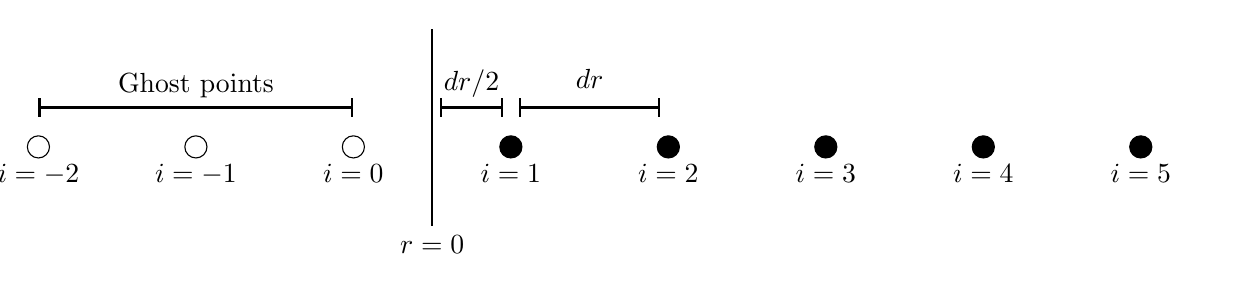
\begin{tikzpicture}
\draw[black] (-3,0) circle (4pt);
\node [below] at (-3,-0.1) {$i=-2$};
\draw[black] (-1,0) circle (4pt);
\node [below] at (-1,-0.1) {$i=-1$};
\draw[black] (1,0) circle (4pt);
\node [below] at (1,-0.1) {$i=0$};
\filldraw[black] (3,0) circle (4pt);
\node [below] at (3,-0.1) {$i=1$};
\filldraw[black] (5,0) circle (4pt);
\node [below] at (5,-0.1) {$i=2$};
\filldraw[black] (7,0) circle (4pt);
\node [below] at (7,-0.1) {$i=3$};
\filldraw[black] (9,0) circle (4pt);
\node [below] at (9,-0.1) {$i=4$};
\filldraw[black] (11,0) circle (4pt);
\node [below] at (11,-0.1) {$i=5$};
\draw[black,thick,|-|] (2.1,0.5) -- (2.9,0.5);
\node[above] at (2.5,0.5) {$dr/2$};
\draw[black,thick,|-|] (3.1,0.5) -- (4.9,0.5);
\node[above] at (4,0.62) {$dr$};
\draw[black,thick] (2,-1) -- (2,1.5);
\node [below] at (2,-1) {$r=0$};
\draw[black,thick,|-|] (-3,0.5) -- (1,0.5);
\node [above] at (-1,0.5) {Ghost points};
\end{tikzpicture}
\end{center}
\caption{Basic grid structure close to $r=0$ showing how the origin is
  staggered.  We show the case of 3 ghost points to the left of the
  origin (for fourth order spatial differencing).}
\label{fig:grid}
\end{figure}


\subsection{Box-in-box grid refinement}

The also code uses ``box-in-box'' type grid refinement.  That is, it
has refinement levels with higher resolution close to the origin set
up at the beginning from the parameter file. The base resolution for
the coarsest grid is set in the parameter file using the parameter
\texttt{dr0}, and the total number of grids is set by the parameter
\texttt{Nl} (\texttt{Nl=1} means a uni-grid run). Higher resolution
grids are set up with refinement factors of two for each level (see
Figure~\ref{fig:BiB1}).  It is important to notice that the grid point
positions at different refinement levels do not coincide because of
the staggering of the origin. \\

\begin{figure}[t]
\begin{center}
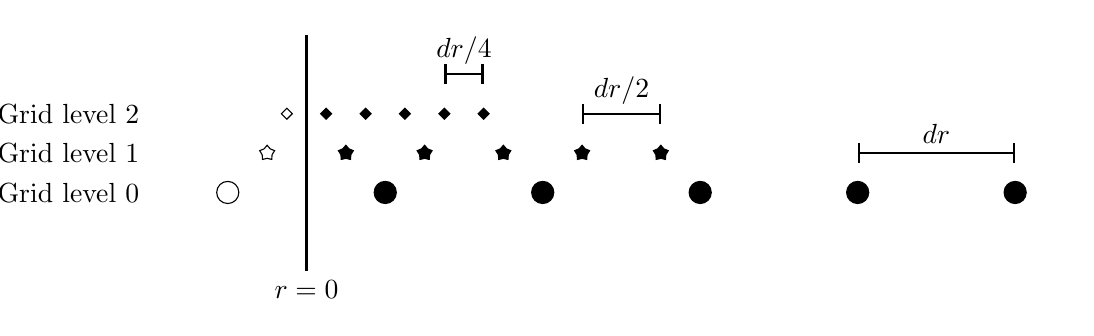
\begin{tikzpicture}
\draw[black,thick] (2,-1) -- (2,2);
\node [below] at (2,-1) {$r=0$};
\draw[black] (1,0) circle (4pt);
\filldraw[black] (3,0) circle (4pt);
\filldraw[black] (5,0) circle (4pt);
\filldraw[black] (7,0) circle (4pt);
\filldraw[black] (9,0) circle (4pt);
\filldraw[black] (11,0) circle (4pt);
\draw[black,thick,|-|] (9,0.5) -- (11,0.5);
\node[above] at (10,0.5) {$dr$};
\node[left] at (0,0) {Grid level 0};
\node[draw,star,scale=0.4] at (1.5,0.5) {};
\node[draw,star,fill=black,scale=0.4] at (2.5,0.5) {};
\node[draw,star,fill=black,scale=0.4] at (3.5,0.5) {};
\node[draw,star,fill=black,scale=0.4] at (4.5,0.5) {};
\node[draw,star,fill=black,scale=0.4] at (5.5,0.5) {};
\node[draw,star,fill=black,scale=0.4] at (6.5,0.5) {};
\draw[black,thick,|-|] (5.5,1) -- (6.5,1);
\node[above] at (6,1) {$dr/2$};
\node[left] at (0,0.5) {Grid level 1};
\node[draw,diamond,scale=0.3] at (1.75,1) {};
\node[draw,diamond,fill=black,scale=0.3] at (2.25,1) {};
\node[draw,diamond,fill=black,scale=0.3] at (2.75,1) {};
\node[draw,diamond,fill=black,scale=0.3] at (3.25,1) {};
\node[draw,diamond,fill=black,scale=0.3] at (3.75,1) {};
\node[draw,diamond,fill=black,scale=0.3] at (4.25,1) {};
\draw[black,thick,|-|] (3.75,1.5) -- (4.25,1.5);
\node[above] at (4,1.5) {$dr/4$};
\node[left] at (0,1) {Grid level 2};
\end{tikzpicture}
\end{center}
\caption{Box-in-box grid refinement close to the origin. Notice that
  the positions of the grid points at different refinement levels do
  not coincide because of the staggering of the origin.}
\label{fig:BiB1}
\end{figure}

When using grid refinement the time step $dt$ is also refined in the
same way, so that a the first refinement level takes twice as many
time steps as the coarsest grid, the second refinement level four
times as many time steps, and so on. There are two important concepts
that should be mentioned here, the operations known as ``restriction''
and ``prolongation''.  Restriction refers to the injection of fine
grid information into a coarser grid once they both reach the same
time level.  Prolongation refers, on the other hand, to the use of
coarse grid information to create new fine grids, which we don't do
here since the grid structure is defined from the beginning.  However,
coarse grid information is still needed in order to give boundary
conditions to the fine grids. \\

In order to understand how the integration in time proceeds let us
consider the case of only two grid levels (if there are more levels
the same procedure is applied recursively). Assuming we already have
initial data for both grid levels, first the coarse grid is advanced
one full time step. After this, the fine grid is advanced two half
time steps until it coincides again with the coarse grid (see
Figure~\ref{fig:BiB2}).  Notice that in order to do this we need to
give boundary data to the fine grid, which is obtained from the coarse
grid via interpolation in both time and space.  At the moment the code
uses cubic interpolation in space, and quadratic interpolation in time
by keeping three coarse time steps in memory (we only need to keep the
data close to the fine grid boundary). This does not work for the very
first steps since we don't have enough coarse time steps yet, so for
the first two fine grid time steps we use linear interpolation in
time. \\

\begin{figure}[h]
\begin{center}
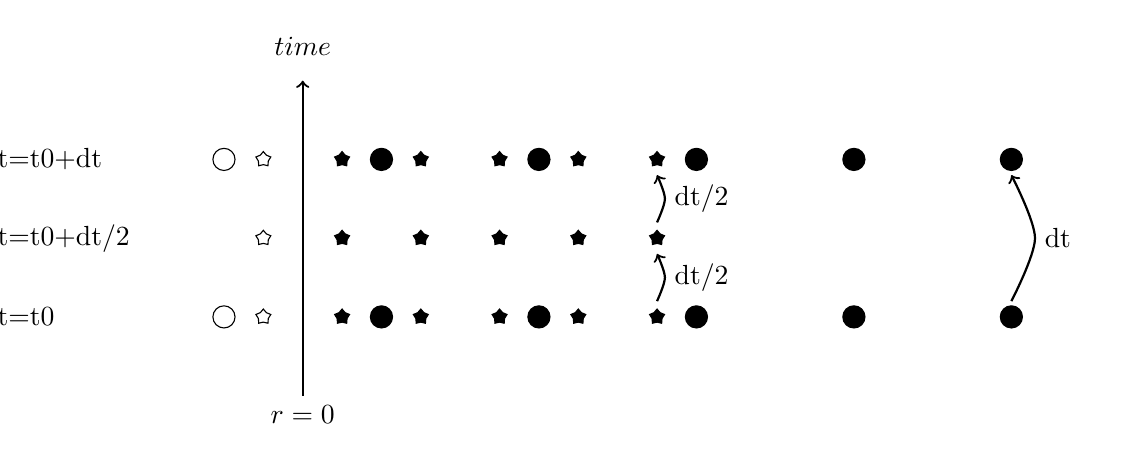
\begin{tikzpicture}
\draw[black,thick,->] (2,-1) -- (2,3);
\node[above] at (2,3.2) {$time$};
\node [below] at (2,-1) {$r=0$};
\draw[black] (1,0) circle (4pt);
\filldraw[black] (3,0) circle (4pt);
\filldraw[black] (5,0) circle (4pt);
\filldraw[black] (7,0) circle (4pt);
\filldraw[black] (9,0) circle (4pt);
\filldraw[black] (11,0) circle (4pt);
\draw[black] (1,2) circle (4pt);
\filldraw[black] (3,2) circle (4pt);
\filldraw[black] (5,2) circle (4pt);
\filldraw[black] (7,2) circle (4pt);
\filldraw[black] (9,2) circle (4pt);
\filldraw[black] (11,2) circle (4pt);
\draw[black,thick,->] plot [smooth] coordinates {(11,0.2) (11.3,1) (11,1.8)};
\node[right] at (11.3,1) {dt};
\node[draw,star,scale=0.4] at (1.5,0) {};
\node[draw,star,fill=black,scale=0.4] at (2.5,0) {};
\node[draw,star,fill=black,scale=0.4] at (3.5,0) {};
\node[draw,star,fill=black,scale=0.4] at (4.5,0) {};
\node[draw,star,fill=black,scale=0.4] at (5.5,0) {};
\node[draw,star,fill=black,scale=0.4] at (6.5,0) {};
\node[draw,star,scale=0.4] at (1.5,1) {};
\node[draw,star,fill=black,scale=0.4] at (2.5,1) {};
\node[draw,star,fill=black,scale=0.4] at (3.5,1) {};
\node[draw,star,fill=black,scale=0.4] at (4.5,1) {};
\node[draw,star,fill=black,scale=0.4] at (5.5,1) {};
\node[draw,star,fill=black,scale=0.4] at (6.5,1) {};
\node[draw,star,scale=0.4] at (1.5,2) {};
\node[draw,star,fill=black,scale=0.4] at (2.5,2) {};
\node[draw,star,fill=black,scale=0.4] at (3.5,2) {};
\node[draw,star,fill=black,scale=0.4] at (4.5,2) {};
\node[draw,star,fill=black,scale=0.4] at (5.5,2) {};
\node[draw,star,fill=black,scale=0.4] at (6.5,2) {};
\draw[black,thick,->] plot [smooth] coordinates {(6.5,0.2) (6.6,0.5) (6.5,0.8)};
\node[right] at (6.6,0.5) {dt/2};
\draw[black,thick,->] plot [smooth] coordinates {(6.5,1.2) (6.6,1.5) (6.5,1.8)};
\node[right] at (6.6,1.5) {dt/2};
\node[right] at (-2,0) {t=t0};
\node[right] at (-2,1) {t=t0+dt/2};
\node[right] at (-2,2) {t=t0+dt};
\end{tikzpicture}
\end{center}
\caption{Time stepping for two refinement levels (for the case of 1
  ghost point).  The coarse grid is first advanced one full time step,
  and after that the fine grid is advanced two half time steps, using
  information from the coarse grid to set up boundary data.}
\label{fig:BiB2}
\end{figure}

Once both grids coincide in time again we inject (restrict) data from
the fine grid back into the coarse grid at those locations that are
covered by both grids.  Notice that if the coarse grid points
coincided with fine grid points one could simply just copy the
information from the fine grid into the coarse grid (though in
practice some kind of average is often used to eliminate high
frequency noise). However, due to the staggering of the origin, our
fine and coarse grids do not coincide, so in practice we interpolate
from the fine grid into the coarse grid (using cubic
interpolation). \\


\subsection{Domain decomposition paralellization}

The code uses a ``domain decomposition'' model for paralellization,
that is, it distributes the full grid among the different
processors. In order to minimize communications between processors,
ghost points are also added to the sides of each grid so that there is
enough information to calculate spatial differences.  Later, at the
end of each time step, these ghost points are ``synchronized'', that
is, information is copied to the ghost points of a given processor
from the corresponding interior points of neighboring processors, see
Figure~\ref{fig:domaindecomp}. \\

\begin{figure}[h]
\begin{center}
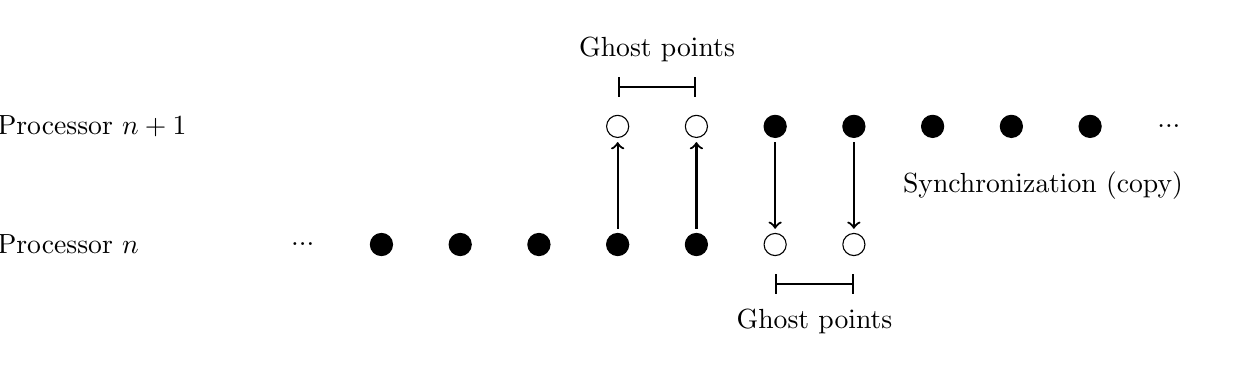
\begin{tikzpicture}
\node at (-5,-1.5) {...};
\filldraw[black] (-4,-1.5) circle (4pt);
\filldraw[black] (-3,-1.5) circle (4pt);
\filldraw[black] (-2,-1.5) circle (4pt);
\filldraw[black] (-1,-1.5) circle (4pt);
\filldraw[black] ( 0,-1.5) circle (4pt);
\draw[black] (1,-1.5) circle (4pt);
\draw[black] (2,-1.5) circle (4pt);
\draw[black] (-1,0) circle (4pt);
\draw[black] ( 0,0) circle (4pt);
\filldraw[black] (1,0) circle (4pt);
\filldraw[black] (2,0) circle (4pt);
\filldraw[black] (3,0) circle (4pt);
\filldraw[black] (4,0) circle (4pt);
\filldraw[black] (5,0) circle (4pt);
\node at (6,0) {...};
\draw[black,thick,|-|] (-1,0.5) -- (0,0.5);
\node [above] at (-0.5,0.7) {Ghost points};
\draw[black,thick,|-|] (1,-2) -- (2,-2);
\node [below] at (1.5,-2.2) {Ghost points};
\node [right] at (-9,-1.5) {Processor $n$};
\node [right] at (-9,0) {Processor $n+1$};
\draw[black,thick,->] (-1,-1.3) -- (-1,-0.2);
\draw[black,thick,->] ( 0,-1.3) -- ( 0,-0.2);
\draw[black,thick,->] (+1,-0.2) -- (+1,-1.3);
\draw[black,thick,->] (+2,-0.2) -- (+2,-1.3);
\node [right] at (2.5,-0.75) {Synchronization (copy)};
\end{tikzpicture}
\end{center}
\caption{Overlapping grids for two processors showing the domain
  decomposition model with the ghost points (in this case two) for
  each processor, and the synchronization operation.}
\label{fig:domaindecomp}
\end{figure}

For simplicity, the number of ghost points used here is the same as
the number used to the left of the origin (see above), and is
controlled by the same parameter \texttt{ghost} (determined at
evolution time). Notice that when we use grid refinement, each grid
level is decomposed in exactly the same way among the same
processors. \\


%%%%%%%%%%%%%%%%%%%%%
%%%   SPACETIME   %%%
%%%%%%%%%%%%%%%%%%%%%

\setcounter{equation}{0}
\section{Spacetime and evolution equations}

\subsection{Spacetime metric}

In the code, the spatial metric is written in the following way:\\
\begin{eqnarray}
dl^2 &=& \psi(r,t)^4 \left( A(r,t) dr^2 + r^2 B(r,t) \: d\Omega^2 \right) \; , \nonumber \\
&=& e^{4 \phi(r,t)} \left( A(r,t) dr^2 + r^2 B(r,t) \: d\Omega^2 \right) \; ,
\label{eq:metric}
\end{eqnarray}
with $d\Omega^2=d\theta^2 + \sin^2 \theta d\varphi^2$ the solid angle
element, and with $\psi = e^\phi$ the conformal factor. The full
spacetime metric takes the form: \\
\begin{equation}
ds^2 = \left(-\alpha^{2} + \beta_{r}\beta^{r} \right) dt^2
+ 2 \beta_{r} dt dr + dl^2 \; ,
\end{equation}
where $\alpha$ is the lapse function and $\beta^{r}$ the shift vector
(which only has a radial component), and where $\beta_r = A \beta^r$. \\


\subsection{Evolution equations}

For the evolution equations, the code uses a
Baumgarte-Shapiro-Shibata-Nakamura (BSSN) formulation adapted to
spherical symmetry.  The specific form of the evolution equations used
here can be found in~\cite{Alcubierre11}. \\

There are two BSSN variants or ``flavors'' controlled by the
parameter \texttt{bssnflavor}, which can take the values
\texttt{lagrangian} or \texttt{eulerian} (the
default is \texttt{bssnflavor=lagrangian}). They refer to the way in which the
shift terms are added to make determinant of the conformal metric
constant along time-lines (lagrangian), or constant along the
normal-lines (eulerian). \\

There is also a parameter that allows one to switch off the evolution
of the spacetime, which is useful in case one wants to evolve some
matter field in a fixed background spacetime. The parameter is called
\texttt{spacetime} and can have the values \texttt{dynamic} or
  \texttt{static} (default is \texttt{spacetime=dynamic}). \\

The main evolution variables (arrays) are:

\begin{list}{}{
\setlength{\leftmargin}{35mm}
\setlength{\labelsep}{10mm}
\setlength{\labelwidth}{20mm}}

\item[\texttt{alpha}] The lapse function $\alpha$.

\item[\texttt{beta}] The contravariant radial shift component $\beta^r$.

\item[\texttt{A}] The conformal radial metric component $\texttt{A}:=\tilde{g}_{rr}$.

\item[\texttt{B}] The conformal radial angular component $\texttt{B}:=\tilde{g}_{\theta \theta}/r^2$.

\item[\texttt{phi}] The conformal factor $\texttt{phi}=\phi$ (see equation~\ref{eq:metric}).

\item[\texttt{KTA}] The mixed radial component of the trace-free
  extrinsic curvature $K^{TF}_{ij}$, \mbox{$\texttt{KTA} :=
    {(K^{TF})^r}_r \equiv K_A$}.

\item[\texttt{KTB}] The mixed angular component of the trace-free
  extrinsic curvature $K^{TF}_{ij}$, \mbox{$\texttt{KTB} :=
    {(K^{TF})^\theta}_\theta \equiv K_B$}.

\item[\texttt{trK}] The trace of the extrinsic curvature \mbox{$\texttt{trK} :=
    {K^m}_m$}.

\item[\texttt{Deltar}] The auxiliary BSSN variable
  \mbox{$\texttt{Deltar} = \Delta^r$}, which is defined as:
\begin{eqnarray}
\Delta^r &:=& \frac{1}{A} \left[ \frac{\partial_r A}{2A} - \frac{\partial_r B}{B}
- \frac{2}{r} \left( 1 - \frac{A}{B} \right) \right] \; , \nonumber \\
&=& \frac{1}{A} \left[ \frac{\partial_r A}{2A} - \frac{\partial_r B}{B}
- 2 r \lambda \right] \; ,
\end{eqnarray}
with $\lambda$ one of the regularization variables (see
Section~\ref{sec:regularization}).

\item[\texttt{dtbeta}] This is the time derivative of the shift:
  $\partial_t \beta = \texttt{dtbeta}$.  When we use advection terms
  for the evolution of the shift (see Section~\ref{sec:shift}),
  $\texttt{dtbeta}$ is not quite the time derivative, and we have
  instead: \mbox{$\partial_t \beta = \texttt{dtbeta} + \beta
    \partial_r \beta$}.

\end{list}

Notice that for the trace free extrinsic curvature one must have
\mbox{$K_A + 2K_B=0$}.  Also, even though the auxiliary BSSN variable
$\Delta^r$ is initially defined in terms of metric derivatives, it is
later evolved independently with its own evolution equation (modified
using the momentum constraint), as required in the BSSN
formulation. \\

The general BSSN formulation allows for a free parameter $\eta$ that
controls how much of the momentum constraint has been added to the
evolution equation for $\Delta^r$. Standard BSSN takes $\eta=2$, and
it can be shown that one needs to take $\eta>1/2$ in order to have a
strongly hyperbolic system. The choice $\eta=2$ guarantees that the
travelling modes associated with the constraints travel at the speed
of light. In the code this is controlled by the parameter \texttt{eta}
with default value equal to 2 (it is not a good idea to change
this). \\

The code also calculates a series of auxiliary geometric quantities
defined as:

\begin{list}{}{
\setlength{\leftmargin}{35mm}
\setlength{\labelsep}{10mm}
\setlength{\labelwidth}{20mm}}

\item[\texttt{psi}] The conformal factor $\texttt{psi}:=\psi=e^\phi$.
  The code also calculates $\texttt{psi2}:=\psi^2$ and
    $\texttt{psi4}:=\psi^4$.

\item[\texttt{chi}] Another form of the conformal factor
  $\texttt{chi}=\chi=1/\psi^2$.  This function is in fact evolved
  instead of $\phi$ if one sets the logical parameter
  \texttt{chimethod=.true.} (by default it is false).  This is useful
  for black hole evolutions as it improves the treatment of the
  central puncture.

\item[\texttt{AB2}] Determinant of the conformal spatial metric
  $\texttt{AB2} := A B^2$.  This should be time independent for
  ``lagrangian'' evolutions, while for ``eulerian'' evolutions it
  should change with time.

\item[\texttt{K2}] Square of the extrinsic curvature:¡
  $\texttt{K2}={K_{ij}}^{ij}=K_A^2 + 2 K_B^2 + ({\rm tr} K)^2/3$.

\item[\texttt{RICA}] Radial mixed component of the spatial Ricci
  tensor $\texttt{RICA}={R^r}_r$.

\item[\texttt{RSCAL}] Spatial Ricci scalar $\texttt{RSCAL}={R^i}_i$.

\end{list}

\vspace{3mm}


%%%%%%%%%%%%%%%%%%%%%%%%%%
%%%   REGULARIZATION   %%%
%%%%%%%%%%%%%%%%%%%%%%%%%%

\setcounter{equation}{0}
\section{Regularization}
\label{sec:regularization}

For regular spacetimes one has to make sure the equations are regular
near $r=0$. There are several important issues about regularization of
the evolution equations at the origin: \\

\subsection{Symmetry conditions at the origin}

The first thing that needs to be taken into account is the symmetry
properties of the different dynamical variables at the origin.  Since
variables must be differentiable at the origin, this implies that
metric variables must behave as:
\begin{eqnarray}
\alpha &\thicksim& \alpha^0 + \mathcal{O}(r^2) \\
\beta^r &\thicksim& \mathcal{O}(r) \\
\phi &\thicksim& \phi^0 + \mathcal{O}(r^2) \\
A &\thicksim& A^0 + \mathcal{O}(r^2) \\
B &\thicksim& B^0 + \mathcal{O}(r^2)
\end{eqnarray}

And since this must hold for all time we must also have:
\begin{eqnarray}
K_A &\thicksim& K_A^0 + \mathcal{O}(r^2) \\
K_B &\thicksim& K_B^0 + \mathcal{O}(r^2)
\end{eqnarray}

Imposing these conditions at the origin is then reduced to asking for
some variables to be odd and others to be even. To do this in practice
we stagger the origin. This means that there is no grid point at the
origin, instead the first grid point is at $r=-dr/2$, the second one
at $r=dr/2$ and so on. This makes it very easy to apply symmetry
boundary conditions, since for an even function $f$ we can simply say
$f_0=+f_1$ and for an odd function $f_0=-f_1$. \\


\subsection{Local flatness at the origin}

This problem is more subtle.  Local flatness can be shown to imply
that, in the above expansions for small r, one must have:
\begin{eqnarray}
A^0 &=& B^0 \; , \\
K_A^0 &=& K_B^0 \; .
\end{eqnarray}

The problem with this is that one now has an over-determined boundary
condition: The derivatives of both $A$ and $B$ must vanish at $r=0$,
plus both functions must be equal, that is, three boundary conditions
for two quantities (and the same happens for $K_A$ and $K_B$). \\

We deal with this problem by introducing the auxiliary variables:
\begin{eqnarray}
\lambda &=& \frac{1}{r^2} \left( 1-\frac{A}{B} \right) \; , \\
K_\lambda &=& \frac{1}{r^2} \left( K_A - K_B \right) \; ,
\end{eqnarray}
which are used to rewrite the problematic terms, and imposing the
extra boundary conditions on $\lambda$ and $K_\lambda$ (basically,
local flatness implies that both are even at $r=0$).  The details of
this procedure can be found in \cite{Alcubierre05,Alcubierre08}. \\


%%%%%%%%%%%%%%%%%%
%%%   MATTER   %%%
%%%%%%%%%%%%%%%%%%

\setcounter{equation}{0}
\section{Matter}
\label{sec:matter}

When we write the Einstein equations in 3+1 form, the components of
the stress-energy tensor that will be important are the energy density,
momentum density and spatial stress tensor as measured by the
so-called Eulerian observers, {\em i.e.} those that move along
the normal direction to the spatial hypersurfaces:
\begin{eqnarray}
\rho &=& n^\mu n^\nu T_{\mu \nu} \; , \\
J_i &=& - n^\mu P_i^\nu T_{\mu \nu} \; , \\
S_{ij} &=& P_i^\mu P_i^\nu T_{\mu \nu} \; ,
\end{eqnarray}
with $n^\mu$ the unit normal vector to the spatial hypersurfaces of
constant coordinate time, and $P^\mu_\nu$ the projector operator onto
these hypersurfaces. \\

Notice that since this code is for spherically symmetric spacetimes,
we in fact only have one component for the momentum density, which the
code takes to be the covariant one (index down): $J_A:=J_r$. Also, we
only have two independent components of the spatial stress tensor
which the code takes with mixed indices (one up, one down): $S_A :=
S^r_r$ and $S_B := S^\theta_\theta$. \\

In the code, these quantities are defined even for vacuum (they are
set to zero), since they are required both in the evolution equations
and for the calculation of the constraints. \\

If you want to add a new matter model, you need to be sure that you
add the appropriate expressions for these quantities in the file
\texttt{src/matter/matter.f90}.  Just have a look at what is already
there to guide you, and try to follow the same conventions. \\

The type of matter used by the code is controlled by the
character-type parameter \texttt{mattertype}.  At the moment it allows
the following values:

\begin{list}{}{
\setlength{\leftmargin}{35mm}
\setlength{\labelsep}{10mm}
\setlength{\labelwidth}{30mm}}

\item[\texttt{vacuum}] There is no matter (this is the default).

\item[\texttt{cosmo}] Cosmological constant.

\item[\texttt{scalar}] Real scalar field.  The scalar field is assumed
  to have a potential whose form is controlled by the parameter
  \texttt{scalarpotential}, which can take the values
  (\texttt{none,phi2,phi4}), corresponding to a free scalar field
  (\texttt{none}), a massive scalar field with a
  potential of the form $V=m^2 \Phi^2/2$
  (\texttt{phi2}), where the mass $m$ is give by the
  parameter \texttt{scalar\_mass}, or a potential of the form
  $V=m^2 \Phi^2/2 + \lambda \Phi^4 / 4$
  (\texttt{phi4}), with the coefficient of the
  self-interaction term given by the parameter
  \texttt{scalar\_lambda}.

\item[\texttt{ghost}] Ghost scalar field. Similar to the scalar field
  above, but the sign of the stress-energy tensor is reversed.

\item[\texttt{complex}] Complex scalar field.  The complex scalar
  field is assumed to have a potential whose form is controlled by the
  parameter \texttt{complexpotential}, which can take the values
  (\texttt{none,phi2,phi4}), corresponding to a free scalar field
  (\texttt{none}), a massive scalar field with a potential of the form
  $V=m^2 |\Phi|^2/2$ (\texttt{phi2}), where the mass $m$ is give by
  the parameter \texttt{complex\_mass}, or a potential of the form
  $V(\phi)=m^2 |\Phi|^2/2 + \lambda |\Phi|^4 / 4$ (\texttt{phi4}),
  with the coefficient of the self-interaction term given by the
  parameter \texttt{complex\_lambda}.

\item[\texttt{nonmin}] Non-minimally coupled scalar field (Note: I
  need to explain this).

\item[\texttt{proca}] Real Proca field. This is essentially
a massive electromagnetic field, with mass given by the
parameter \texttt{proca\_mass}.

\item[\texttt{complexproca}] Complex Proca field. This is a complex
  Proca field, with mass given by the parameter \texttt{cproca\_mass}.

\item[\texttt{dirac}] Dirac spinor field.

\item[\texttt{electric}] Electric field.

\item[\texttt{fluid}] Perfect fluid.

\item[\texttt{dust}] Dust (perfect fluid with zero pressure).

\end{list}

Any new type of matter model should be added to the list of allowed
values for this parameter in the file \texttt{param.f90}. Notice that
the code allows one to have several different types of matter at the
same time, the corresponding stress-energy tensors are just added
together. For example, if you want to have a real scalar field and a
complex scalar field evolving together you can add the following line
to the parameter file: \\

\texttt{mattertype = scalar,complex} \\

Similarly, for a charged complex scalar field you must have: \\

\texttt{mattertype = complex,electric} \\

\vspace{3mm}


%%%%%%%%%%%%%%%%%%%%%%%
%%%   CONSTRAINTS   %%%
%%%%%%%%%%%%%%%%%%%%%%%

\setcounter{equation}{0}
\section{Constraints}
\label{sec:constraints}

\subsection{Hamiltonian and momentum constraints}

When required for output, the code calculates the Hamiltonian and
momentum constraints and saves them in the arrays \texttt{ham} and
\texttt{mom}.  Notice that since we are in spherical symmetry, the
momentum constraint only has a non-zero radial component. \\

The expression used for the Hamiltonian constraint is:
\begin{equation}
\texttt{ham} := H = R - \left( K_A^2 + 2 K_B^2 \right) + \frac{2}{3} \: {\rm tr} K
- 16 \pi \rho \;,
\end{equation}
with $R$ the spatial Ricci scalar, and $\rho$ the energy density of
matter. \\

For the radial (covariant) momentum constraint we have:
\begin{equation}
\texttt{mom} := M_r = \partial_r K_A - \frac{2}{3} \: \partial_r {\rm tr} K
+ 6 K_A \: \partial_r \phi + r^2 \left( \frac{\partial_r B}{B} + \frac{2}{r} \right)
- 8 \pi J_A \; ,
\end{equation}
with $\phi$ the conformal factor and $J_A$ the covariant radial
component of the momentum density. \\

Notice that for an exact solution both these constraints should be
zero, so monitoring their behaviour, and particularly how they
approach zero as we increase the resolution, gives us information
about the accuracy of the code. \\


\subsection{BSSN extra constraint}

The BSSN formalism requires the introduction of an auxiliary variable
$\Delta^r$ defined in terms of derivatives of the conformal metric
components (see~\cite{Alcubierre11}).  This is then promoted
to an independent variable, and its evolution equation is modified
using the momentum constraint. \\

We therefore end up with a new constraint related to the definition of
$\Delta^r$ and stored for output int he array \texttt{CDeltar}:
\begin{equation}
\texttt{CDelatr} := A \Delta^r - \left( \frac{\partial_r A}{2A} -
\frac{\partial_r B}{B} - 2 r \lambda \right) \; ,
\end{equation}
with $\lambda$ a regularization variable (see below). Again, this
quantity should be zero for an exact solution. \\


\subsection{Regularization constraints}

Finally, for the regularization procedure we need to introduce two
more auxiliary variables that again are evolved independently so we
have two more constraints coming from their definitions that are
saved for output in the arrays \texttt{Clambda} and \texttt{CKlambda}:
\begin{eqnarray}
\texttt{Clambda} &:=& r^2 \lambda - \left( 1 - \frac{A}{B} \right) \; , \\
\texttt{CKlambda} &:=& r^2 K_\lambda - \left( K_A - K_B \right) \; .
\end{eqnarray}

\vspace{3mm}


%%%%%%%%%%%%%%%%%%%%%%%%%%%%%%
%%%   SLICING CONDITIONS   %%%
%%%%%%%%%%%%%%%%%%%%%%%%%%%%%%

\setcounter{equation}{0}
\section{Slicing conditions}
\label{sec:slicing}

The slicing condition is controlled by the parameter \texttt{slicing}, which at the
moment can take one of the following values (default is \texttt{slicing=harmonic}):

\begin{list}{}{
\setlength{\leftmargin}{35mm}
\setlength{\labelsep}{10mm}
\setlength{\labelwidth}{20mm}}

\item[\texttt{static}] The lapse remains static at its initial value and does not evolve.

\item[\texttt{harmonic}] This is a harmonic-type slicing condition of the form:
\begin{equation}
\partial_t \alpha = - \alpha^2 f \: {\rm tr} K + \beta^r \partial_r \alpha \; ,
\end{equation}
where $f$ is a real positive number controlled by the parameter
\texttt{gauge\_f} (default is \texttt{gauge\_f=1}). True harmonic
slicing really corresponds to \texttt{gauge\_f=1}, but here we allow
any positive real number.  This is a hyperbolic slicing condition
corresponding to a speed of propagation of the gauge given by
$\sqrt{f}$.

\item[\texttt{1+log}] This is a slicing condition of the 1+log family,
  which is very similar to the harmonic family above:
\begin{equation}
\partial_t \alpha = - \alpha f \: {\rm tr} K + \beta^r \partial_r \alpha \; ,
\end{equation}
where again $f$ is a positive real number controlled by the same
parameter \texttt{gauge\_f}.  Standard 1+log slicing corresponds to 
\texttt{gauge\_f=2} (though as mentioned above the default value is 1).


\item[\texttt{shockavoid}] This corresponds to the family of shock
  avoiding slicing conditions, which is similar to the 1+log
  condition above but with $f(\alpha)$ a function given by (see
    comments in file \texttt{src/geometry/auxiliary\_geometry.f90}):
\begin{equation}
f(\alpha) = 1 + k/\alpha^2 \; .
\end{equation}

\item[\texttt{maximal}] This is maximal slicing which corresponds to
  the condition that the trace of the extrinsic curvature remains
  equal to zero during evolution (which guarantees that the spatial
  volume elements remain constant), and which implies that the lapse
  must satisfy the following elliptic equation:
\begin{equation}
\nabla^2 \alpha = \alpha K_{ij} K^{ij} + 4 \pi \alpha  \left( \rho + {\rm tr} S \right) \; .
\end{equation}
In spherical symmetry the Laplacian operator reduces to:
\begin{equation}
\nabla^2 = \partial_r^2 + \left( \frac{2}{r} - \frac{\partial_r A}{2A} 
+ \frac{\partial_r B}{B} + 2 \: \partial_r \phi \right) \partial_r \; .
\end{equation}


\end{list}

\vspace{3mm}

Notice that the choices \texttt{harmonic}, \texttt{1+log} and
\texttt{shockavoid} are special cases of the Bona-Masso family of
slicing conditions that has the general form:
\begin{equation}
\partial_t \alpha = - \alpha^2 f(\alpha) {\rm trK} + \beta^r \partial_r \alpha\; .
\end{equation}
with $f(\alpha)$ an arbitrary (positive) function of the lapse.
 
\vspace{5mm}

The initial value of the lapse can also be controlled by the parameter
\texttt{ilapse} which can take the values (default
\texttt{ilapse=none}):

\begin{list}{}{
\setlength{\leftmargin}{35mm}
\setlength{\labelsep}{10mm}
\setlength{\labelwidth}{20mm}}

\item[\texttt{none}] The initial lapse it first set to 1, but can
  later be modified by initial data routines and will not be touched
  after this.

\item[\texttt{one}] The initial lapse is set to 1 again AFTER all
  initial data routines have been called.

\item[\texttt{isotropic}] The initial lapse it set to
  $\alpha=2/\psi-1$ after all initial data routines have been called,
  with $\psi$ the conformal factor.  Notice that this is the correct
  value of the lapse for a static Schwarzschild spacetime in isotropic
  coordinates, but we can use it for any type of initial data and it
  should still result in a lapse that keeps the spacetime
  approximately static far away.

\item[\texttt{psiminus2}] The initial lapse is set to
  $\alpha=1/\psi^2$ after all initial data routines have been called,
  with $\psi$ the conformal factor. This is useful for black hole
  evolutions where $\psi$ becomes infinite at the origin, and results
  in a ```pre-collapsed'' initial lapse that is already zero and
  smooth at $r=0$.

\item[\texttt{psiminus4}] Similar to the case above, but sets the
  initial lapse to $\alpha=1/\psi^4$.

\end{list}

\vspace{5mm}

There is also the possibility of adding a Gaussian to the initial
value of the lapse. This is useful for perturbing the initial data and
causing interesting gauge dynamics.  This is controlled by the
parameters:

\begin{list}{}{
\setlength{\leftmargin}{35mm}
\setlength{\labelsep}{10mm}
\setlength{\labelwidth}{20mm}}

\item[\texttt{lapsegauss}] Logical parameter that if set to
  \texttt{.true.} adds a Gaussian to the initial lapse (default is
  \texttt{.false.}).

\item[\texttt{lapse\_a0}] Amplitude of Gaussian.

\item[\texttt{lapse\_r0}] Center of Gaussian.

\item[\texttt{lapse\_s0}] Width of Gaussian.

\end{list}

\vspace{3mm}


%%%%%%%%%%%%%%%%%%%%%%%%%%%%
%%%   SHIFT CONDITIONS   %%%
%%%%%%%%%%%%%%%%%%%%%%%%%%%%

\setcounter{equation}{0}
\section{Shift conditions}
\label{sec:shift}

Notice that since we are in spherical symmetry the shift vector only
has a radial component.  The shift condition is controlled by the
parameter \texttt{shift}, which at the moment can take one of the
following values (default is \texttt{shift=none}):

\begin{list}{}{
\setlength{\leftmargin}{45mm}
\setlength{\labelsep}{10mm}
\setlength{\labelwidth}{30mm}}

\item[\texttt{none}] There is no shift, and all shift terms in the
  evolution equations are ignored.  This is the default.

\item[\texttt{zero}] The shift is set to zero, but all the shift terms
  in the evolution equations are calculated.  This is useful for
  testing.

\item[\texttt{static}] The shift is non-zero but it does not evolve in
  time. Again, useful for testing.

\item[\texttt{Gammadriver1}] Parabolic Gamma-driver shift.  The shift
  condition is given by:
\begin{equation}
\partial_t \beta^r = \xi \partial_t \Delta^r \; .
\end{equation}

\item[\texttt{Gammadriver2}] Standard second order hyperbolic
  Gamma-driver shift.  The shift condition is given by:
\begin{equation}
\partial^2_t \beta^r = \xi \partial_t \Delta^r - \eta \partial_t \beta^r \; .
\end{equation}
In the code this is written in second order form as:
\begin{eqnarray}
\partial_t \beta^r &=& \cal{B} \; , \\
\partial_t \cal{B} &=& \xi \partial_t \Delta^r - \eta \cal{B} \; .
\end{eqnarray}

This is in fact the standard Gamma-driver used in most BSSN codes.
Notice that in the code ${\cal B}$ is in fact called \texttt{dtbeta}.

\end{list}

\vspace{3mm}

The Gamma-driver shift conditions above relate the evolution of the
shift to that of the BSSN auxiliary variable $\Delta^r$. The values of
the coefficients $\xi$ and $\eta$ are controlled with the real
parameters \texttt{drivercsi} and \texttt{drivereta}.  There is also
the logical parameter \texttt{driveradv} which if set to
\texttt{.true.}  modifies the Gamma driver conditions by adding
advection terms on the shift (by default it is \texttt{.false.}). \\

Just as in the case of the lapse, there is the possibility of adding a
Gaussian to the initial value of the shift. This is useful for
perturbing the initial data and causing interesting gauge dynamics.
This is controlled by the parameters:

\begin{list}{}{
\setlength{\leftmargin}{35mm}
\setlength{\labelsep}{10mm}
\setlength{\labelwidth}{20mm}}

\item[\texttt{shiftgauss}] Logical parameter that if set to
  \texttt{.true.} adds a Gaussian to the initial shift (default is
  \texttt{.false.}).

\item[\texttt{shift\_a0}] Amplitude of Gaussian.

\item[\texttt{shift\_r0}] Center of Gaussian.

\item[\texttt{shift\_s0}] Width of Gaussian.

\end{list}

\vspace{3mm}


%%%%%%%%%%%%%%%%%%%%%%%%%%%%%%%
%%%   BOUNDARY CONDITIONS   %%%
%%%%%%%%%%%%%%%%%%%%%%%%%%%%%%%

\setcounter{equation}{0}
\section{Boundary conditions}
\label{sec:boundary}

The outer boundary conditions for the evolution are controlled by the
character-type parameter \texttt{boundary}, which at the moment can
take one of the following values (the default is \texttt{flat}):

\begin{list}{}{
\setlength{\leftmargin}{35mm}
\setlength{\labelsep}{10mm}
\setlength{\labelwidth}{25mm}}

\item[\texttt{none}] No boundary condition is applied.  The sources are
  applied all the way to the boundary using one-sided differences.

\item[\texttt{static}] The sources are set to zero at the boundary.
  This is done only for evolving arrays that are not declared with the
  keyword \texttt{NOBOUND}.

\item[\texttt{flat}] The sources at the boundary are copied from their
  value one grid point in. This is done only for evolving arrays that
  are not declared with the keyword \texttt{NOBOUND}.

\item[\texttt{radiative}] Outgoing-wave boundary condition. This is
  somewhat more involved as it uses some information from eigenfields
  and eigenspeeds, and works quite well in practice.

\item[\texttt{constraint}] Constraint preserving boundary condition.
This condition uses information from the constraints in order to avoid
introducing constraint violations at the boundary.

\end{list}

\vspace{3mm}

Notice that all the boundary conditions are always applied at the
level of the source terms, and are applied only for some of the
evolving arrays and not all of them.  In general, evolving arrays that
are declared with the keyword \texttt{NOBOUND} have no need for a
boundary condition since their source terms can be calculated all the
way to the boundary. \\

Static and flat boundary conditions are applied in the automatically
generated file \linebreak \texttt{src/auto/simpleboundary.f90}.  The
radiative and constraint preserving boundary conditions are explained
with more detail below.


\subsection{Radiative boundaries}

In this case we apply outgoing wave boundary conditions taking into
account information about the characteristic structure of the
evolution system.  For the case of the geometric boundaries we apply
the radiative boundary condition only to the evolving arrays
(\texttt{trK,KTA,Klambda}), and when we are using a shift condition of
the Gammadriver family also to \texttt{dtbeta}.  For matter variables
(for example scalar fields), radiative boundaries must be coded in
their respective source routines. Here we will explain in some detail
how the radiative boundaries are applied to the geometric variables,
since they are somewhat involved. \\

The characteristic structure of the BSSN system in spherical symmetry
is analysed in detail in~\cite{Alcubierre15}. For the case of zero or
static shift, one finds that there are two families of travelling
modes: One family associated with the slicing condition that travels
with the gauge speed $\alpha \sqrt{f/A}$, with $f(\alpha)$ the
Bona-Masso function that in the code is controlled by the parameter
\texttt{gauge\_f}, and a second family whose speed depends on the
multiple of the constraints that has been added to the evolution
equation for $\Delta^r$, which in the code is controlled by the
parameter \texttt{eta}.  For standard BSSN (\texttt{eta=2}) the second
family in fact travels at the speed of light, but these modes are NOT
associated with gravitational waves (there are no gravitational waves
in spherical symmetry), but rather with the violation of the
constraints. \\

From the characteristic analysis one can show that the trace of the
extrinsic curvature ${\rm tr} K$ is a pure gauge quantity associated
with the slicing condition.  For the boundary condition we then assume
that far away ${\rm tr} K$ behaves as an outgoing spherical wave with
speed $v_f \sim \sqrt{f}$:
\begin{equation}
{\rm tr} K \sim g(r - v_f t)/r \; ,
\end{equation}
with $g$ an arbitrary wave profile.  This can easily be shown to imply
that:
\begin{equation}
\partial_t {\rm tr} K \sim - v_f \left( \partial_r {\rm tr} K
+ {\rm tr} K / r \right) \; .
\end{equation}
This is the radiative boundary condition used in the code for ${\rm
  tr} K$ (except for maximal slicing when we just set ${\rm tr} K=0$
everywhere).  It works remarkably well and results in very small
reflections from the boundary.~\footnote{Notice that a similar
  boundary condition can be used for some matter fields, for example
  real and complex scalar fields, but assuming that the outgoing
  spherical waves travel at the speed of light.} \\

\vspace{3mm}

In order to obtain a boundary condition for $K_A$ (\texttt{KTA} in the
the code) we use a similar idea, but somewhat more involved. From the
characteristic analysis one also finds that the eigenfields that move
at the speed of light for $\eta=2$ mentioned above (associated with
the constraints) are related to $K_A - 2/3 \; {\rm tr} K$ (this
combination is in fact the sum of the outgoing and incoming
eigenfields).  It is clear that the outgoing eigenfield will behave as
an outgoing spherical wave moving at the speed of light, while the
incoming field should be small (it will not be zero since they are
coupled through source terms).  So, if we assume to first
approximation that this combination behaves as:
\begin{equation}
K_A - 2/3 \; {\rm tr} K \sim h(r - v_l t)/r \; ,
\end{equation}
with $v_l \sim 1$ the speed of light far away and $h$ some wave profile,
we find that
\begin{equation}
\partial_t \left( K_A - 2/3 \; {\rm tr} K \right)
\sim - \left[ \partial_r \left( K_A - 2/3 \; {\rm tr} K \right)
+ \left( K_A - 2/3 \; {\rm tr} K \right) / r \right] \; .
\end{equation}
And combining this with the boundary condition for ${\rm tr} K$ above, we
finally find:
\begin{equation}
\partial_t K_A \sim - \left( \partial_r K_A + K_A / r \right) 
- 2/3 \left( v_f - 1 \right)
\left( \partial_r {\rm tr} K + {\rm tr} K / r \right)\; .
\end{equation}
This boundary condition again turns out to be very well-behaved, and
results in very small reflections at the boundary, but it will violate
the constraints (see the following Section).  Notice also that $K_A$
and the regularization variable $K_\lambda$ are closely related to
each other, so having a boundary condition for $K_A$ immediately gives
us a boundary condition for $K_\lambda$. \\

\vspace{3mm}

The last variable to consider is the BSSN function $\Delta^r$.  In
practice we have found that when the shift is zero, or non-zero but
time-independent, or if we are using the parabolic shift condition
\texttt{shift=Gammadriver1}, we can just calculate the source for
$\Delta^r$ all the way to the boundary using one-sided differences
and this results in a stable and well-behaved evolution.  For the
\texttt{shift=Gammadriver2} shift condition the sources for $\Delta^r$
can still be calculated all the way to the boundary, but we now need
to impose a boundary condition on the time derivative of the shift
$\cal{B}$ (which in the code is called \texttt{dtbeta}).  \\

The characteristic analysis for the lagrangian case when we take
\texttt{shift=Gammadriver2} is not very difficult, but for the
eurlerian case it becomes much more complicates, so in the code the
boundary conditions assume that we always use the lagrangian
formulation. In that case it turns out that the shift eigenfields are
related to the quantity ${\cal B} + Q \partial_r \alpha$, with $Q$
given far away as $Q=v_\xi^2/(v_\xi^2 - v_f^2)$, and where $v_\xi \sim
\sqrt{4 \xi/3}$ is the shift gauge speed and $v_f \sim \sqrt{f}$ the
lapse gauge speed defined above. Notice that $Q$ diverges when $v_f =
v_\xi$, which happens for example for pure harmonic slicing and the
standard Gamma driver shift, in which case we have $v_f=v_\xi=1$.
This is a flaw of the standard Gamma driver shift condition, the
characteristic structure becomes ill-defined in this case. However,
the boundary condition below should still work in this case. \\

We now assume that far away we have:
\begin{equation}
{\cal B} + Q \partial_r \alpha \sim u(r - v_\xi t)/r \; ,
\end{equation}
One can show that the above assumption then implies:
\begin{equation}
\partial_t {\cal B} \sim - v_\xi \left( \partial_r {\cal B} + {\cal B} / r \right)
- \frac{v_\xi^2}{v_\xi + v_f} \left( \partial^2_r \alpha + \partial_r \alpha / r \right) \: .
\end{equation}
We can now apply this condition at the boundary, using one-sided
derivatives for the lapse, and it works quite well.  But we still need
to make one final transformation.  The above expression has two
drawbacks: First, it involves second derivatives of the lapse, which
at the boundary are less accurate and should be avoided if possible,
but worse, even though it works well for travelling waves, for
stationary solutions with a non-trivial lapse it introduces a drift at
the boundary.  Both these drawbacks can be addressed if we notice
that, for an outgoing travelling wave the incoming slicing eigenfield
should be very small.  From the characteristic analysis we find that
this implies $\partial_r \alpha \sim v_f \: {\rm tr} K$.  We can
then rewrite the above expression as:
\begin{equation}
\partial_t {\cal B} \sim - v_\xi \left( \partial_r {\cal B} + {\cal B} / r \right)
- \frac{v_f v_\xi^2}{v_\xi + v_f}
\left( \partial_r {\rm tr} K + {\rm tr} K / r \right) \: .
\end{equation}
This expression does not involve second derivatives of the lapse, and
has the advantage that for static solutions ${\rm tr} K$ vanishes, so
it should reduce the drift at the boundary. This boundary condition
works surprisingly well and is the one used in the code.


\subsection{Constraint preserving boundaries}

The radiative boundaries explained above introduce constraint
violations at the boundaries, which arise directly from the condition
applied to $K_A$. Here we use a method based on~\cite{Alcubierre15},
but modified in a way that makes it both simpler and more robust. \\

We start from the fact, mentioned above, that the incoming and outgoing modes
associated with the constraints, $\omega^+_l$ and $\omega^-_l$, are such that
\begin{equation}
\omega^+_l + \omega^-_l = K_A - 2/3 \; {\rm tr} K \; ,
\end{equation}
which clearly implies:
\begin{equation}
\partial_t K_A = 2/3 \; \partial_t {\rm tr} K
+ \partial_t \left( \omega^+_l + \omega^-_l \right) \; .
\end{equation}
Assume now that the time derivative of ${\rm tr} K$ at the boundary
has already been obtained from the radiative condition above.  This
will not in itself violate the constraints as ${\rm tr} K$ is pure
gauge. \\

It turns out that the time derivative of $\left( \omega^+_l +
\omega^-_l \right)$ can be written in terms of the constraints in such
a way that if one then asks for the constraints to vanish this
quantity evolves only through source terms (that is, no derivatives of
the extrinsic curvature or second derivatives of the metric). The
resulting expression is not terribly complicated but it is not
particularly illuminating either, so I will not write it here. \\

We can the simply use the expression above as a boundary condition for
$K_A$ that will not violate the constraints. In practice, we find that
as a pulse of constraint violation reaches the boundary, it gets
reflected with an amplitude of roughly the same size, and this
converges away with increased resolution. \\


%%%%%%%%%%%%%%%%%%%%%%%%
%%%   INITIAL DATA   %%%
%%%%%%%%%%%%%%%%%%%%%%%%

\setcounter{equation}{0}
\section{Initial data}
\label{sec:initial}

The type of initial data is controlled by the character-type parameter
\texttt{idata}.  If you add a new type of initial data it should be
appended to the list of allowed values for this parameter in the file
\texttt{src/base/param.f90}.  You should also add a corresponding call
to your initial data routine in the file
\texttt{src/base/initial.f90}. \\

There are in fact many more initial data types than the ones discussed
here that have been added through the years (like charged boson stars,
Proca stars, Dirac stars, etc.). Have a look at the file
\texttt{src/base/param.f90} to see the values allowed by
\texttt{idata}, and the corresponding routines that calculate them
(routines with names that typically start with \texttt{idata\_} and
can be found in the directories \texttt{src/geometry} and
\texttt{src/matter}). \\

Simple types of vacuum initial data already there are:

\begin{list}{}{
\setlength{\leftmargin}{55mm}
\setlength{\labelsep}{10mm}
\setlength{\labelwidth}{50mm}}

\item[\texttt{idata=minkowski}] The initial metric is simply set to
  Minkowski and the extrinsic curvature is set to zero.  Notice that
  one can still have non-trivial gauge evolution if one adds a
  Gaussian perturbation to the initial lapse (see
  Section~\ref{sec:slicing}).

\item[\texttt{idata=schwarzschild}] The initial metric is set to that
  corresponding to a Schwarzschild black hole in isotropic coordinates:
  $A=B=1$, $\psi=1 + M/(2r^2)$. Here $M$ is the mass of the black
  hole controlled by the parameter \texttt{BHmass} (default is 1).
  The initial extrinsic curvature is set to zero.

\item[\texttt{idata=trumpetBH}] The initial data corresponds to a
  Schwarzschild black hole in the so-called ``trumpet'' gauge. This
  data is not analytic and must be solved numerically.

\item[\texttt{idata=reissnernordstrom}] The initial data corresponds
to a Reissner-Nordstrom charged black hole.

\end{list}

\vspace{5mm}

There is also already some initial data with matter for the case of
real or complex scalar fields:

\begin{list}{}{
\setlength{\leftmargin}{55mm}
\setlength{\labelsep}{10mm}
\setlength{\labelwidth}{45mm}}

\item[\texttt{idata=scalarpulse}] The initial data is a simple
  Gaussian pulse of a real scalar field.  The amplitude, center and
  width of the Gaussian are controlled by the parameters
  \texttt{scalar\_a0}, \texttt{scalar\_r0}, \texttt{scalar\_s0}.  The
  initial data is assumed to be time-symmetric, and the Hamiltonian
  constraint is solved for the conformal factor.

\item[\texttt{idata=ghostpulse}] Similar as the case above, but for a
  ghost scalar field.

\item[\texttt{idata=complexpulse}] The initial data is a simple
  Gaussian pulse of a complex scalar field.  The amplitude, center and
  width of the Gaussian, for the real and imaginary parts, are
  controlled by the parameters \texttt{complexR\_a0},
  \texttt{complexR\_r0}, \texttt{complexR\_s0} and
  \texttt{complexI\_a0}, \linebreak \texttt{complexI\_r0},
  \texttt{complexI\_s0}, respectively.  The initial data is assumed to
  be time-symmetric, and the Hamiltonian constraint is solved for the
  conformal factor.

\item[\texttt{idata=bosonstar}] The initial data corresponds to a
  Boson Star.  This requires complex scalar field matter with non-zero
  mass. For this initial data one must set the central value of the
  real part of the scalar field with the parameter
  \texttt{complex\_phi0}, and one must also give two bracketing values
  of the frequency with the parameters \texttt{omega\_left} and
  \texttt{omega\_right}.  Notice that these values need to be given
  with high precision or the solution will fail.

\end{list}

In order to restart from a checkpoint file, we must have: \\

\texttt{idata=checkpoint} 

\vspace{3mm}


%%%%%%%%%%%%%%%%%%%%
%%%   HORIZONS   %%%
%%%%%%%%%%%%%%%%%%%%

\setcounter{equation}{0}
\section{Apparent horizons}
\label{sec:horizons}

For spacetimes that contain black holes, either from the initial data
or through gravitational collapse during the evolution, the code can
look for apparent horizons.  Since we are in spherical symmetry, this
in fact reduces to finding a zero of the expansion for null light rays
given by:
\begin{equation}
\Theta := \frac{1}{\psi^2 A^{1/2}} \left( \frac{2}{r} + \frac{\partial_r B}{B}
+ 4 \: \partial_r \phi \right) - 2 K_B \; ,
\end{equation}
where $\psi$ is the conformal factor.  An apparent horizon will
correspond to the outermost value of $r$ for which the expansion
$\Theta$ is equal to zero. \\

The code will look for apparent horizons whenever the logical
parameter \texttt{ahfind} is set to \texttt{.true.} (by default it is
\texttt{.false.}).  It will look for horizons every certain number of
time steps, controlled by the value of the integer parameter
\texttt{ahfind\_every} (by default 1). \\

Once it locates a horizon, it will output its position as a function
of time in the file \texttt{ah\_radius.tl} (if no horizon is found
this value is 0). It will also output its physical area, its
Schwarzschild radius, and its mass to the files \texttt{ah\_area.tl},
\texttt{ah\_schw.tl} and \texttt{ah\_mass.tl}, respectively.  Notice
that the mass of the apparent horizon is defined in terms of its area
$A$ as: $M_{AH} := \sqrt{ A/16 \pi}$. \\

It is sometimes useful to know the value of the lapse at the position
of the horizon, so the code also outputs this value in the file
\texttt{ah\_alpha.tl}. \\


%%%%%%%%%%%%%%%%%%%%%%%%%%
%%%   ANALYSIS TOOLS   %%%
%%%%%%%%%%%%%%%%%%%%%%%%%%

\setcounter{equation}{0}
\section{Other analysis tools}
\label{sec:analysis}

The code can also calculate many other quantities for analysis that
are not listed here, such as for example the total Schwarzschild-like
mass (\texttt{mass\_sch}), the total integrated mass
(\texttt{mass\_int}), the areal radial coordinate (\texttt{r\_area}),
the expansion of null geodesics, the Weyl tensor, the 4D Ricci scalar,
the curvature invariants $I$ and $J$, total conserved charges for
different types of fields, etc. \\

I will not enlist all those quantities here as they continue to grow
all the time, but have a look at the files
\texttt{src/geometry/analysis\_geometry.f90} and
\texttt{src/matter/matter\_geometry.f90}. In order to calculate any
such quantities you MUST ask for output of them in the parameter file.



%%%%%%%%%%%%%%%%%%%%%%%%%%%%%
%%%   NUMERICAL METHODS   %%%
%%%%%%%%%%%%%%%%%%%%%%%%%%%%%

\setcounter{equation}{0}
\section{Numerical methods}
\label{sec:numerics}

\subsection{Time integration}

For the time integration the code uses a method of lines, where the
time integration and spatial differentiation are considered
independent of each other. \\

For the evolution of the field variables we can use one of two
methods:

\begin{enumerate}

\item Standard fourth order Runge-Kutta.

\item 3-step iterative Crank-Nicholson scheme (ICN).  The ICN scheme for
N iterations is defined as follows (with $S(f)$ the source term of the
evolution equation):
\begin{eqnarray}
f_0  &=&  f(t) \; , \\
f_{i+1} &=&  f_0 + dt/2 \; S(f_i)  \qquad \textrm{i from 1 to N-1} \; , \\
f_N &=&  f_0 + dt \; S(f_{N-1}) \; , \\
f_t+dt &=& f_N
\end{eqnarray}

That is, we do $N-1$ half steps starting always from $f(t)$ but
evaluating the source term using the results from the previous step.
Finally, we do one last full step.  Doing only 2 ($N=2$) steps is
enough for second order accuracy, but we need to do at least 3 ($N=3$)
for stability.  ICN is a rather robust method that can be applied to
non-linear systems of equations, but it is somewhat dissipative.

\end{enumerate}

The choice of the integration method is done through the parameter
\texttt{integrator} which can take the values \{\texttt{rk4,icn}\}. \\


\subsection{Spatial differencing}

For spatial differentiation we can use either second or fourth order
differencing (I have also added sixth and eight order, but this is
ussually not needed as the time integration is at most fourth order).
Close to the outer boundaries we in fact reduce the differencing
always to second order.  The choice of the differencing order is
controlled by the parameter \texttt{order} which can take the values
\{\texttt{two,four}\}. \\


\subsection{Dissipation}

The code uses Kreiss-Oliger type dissipation to improve stability.
Often one can turn this off and things will still work, but is seems
to be important for scalar field evolutions and also to keep a black
hole spacetime stable for a long time. The dissipation of the
geometric variables is controlled by the parameter \texttt{geodiss},
and the dissipation for the scalar field (both real and complex) is
controlled by the parameter \texttt{scalardiss}. Both are set by
default to a value of 0.01. Other type of matter fields have similar
dissipation parameters (\texttt{nonmindiss}, \texttt{procadiss},
etcetera).\\


%%%%%%%%%%%%%%%%%%%%%%%%%%%%%%
%%%   LIST OF PARAMETERS   %%%
%%%%%%%%%%%%%%%%%%%%%%%%%%%%%%

\section{List of main code parameters}
\label{sec:parameters}

Here is a list of the main code parameters with their default values
and ranges when applicable.  For a list of all declared parameters see
the file \texttt{src/base/param.f90}.  But do notice that some of the
``parameters'' declared in \texttt{param.f90} should not be fixed in
the parameter file since they are in fact defined at run time. \\

There are many more parameters that are not mentioned here,
particularly related to new matter models or initial data routines.
Have a look at the file \texttt{src/base/param.f90} where they are
defined, they are usually explained in the comments). \\

\begin{itemize}

\item Grid parameters:

\begin{list}{}{
\setlength{\leftmargin}{60mm}
\setlength{\labelsep}{10mm}
\setlength{\labelwidth}{50mm}}

\item[\texttt{dr0 (real(8))}] Spatial interval for base (coarsest) (default 1.0).

\item[\texttt{Nrtotal (integer)}] Total number of grid points for base grid (default
  10).

\item[\texttt{Nl (integer)}] Number of refinement levels (default
  1).

\item[\texttt{ghost (integer)}] Number of ghost zones (default 0).
  Should NOT be fixed in the parameter file.

\item[\texttt{intorder (integer)}] Order of interpolation (default
  3).  Don't change this unless you know what you are doing!

\item[\texttt{boundary (character)}] Type of outer boundary condition.
  Can take the following values: \texttt{none}, \texttt{static},
  \texttt{flat}, \texttt{radiative} (default \texttt{flat}).

\end{list}

\item Time stepping parameters:

\begin{list}{}{
\setlength{\leftmargin}{60mm}
\setlength{\labelsep}{10mm}
\setlength{\labelwidth}{50mm}}

\item[\texttt{dt0 (real(8))}] Time step for base (coarsest) grid
  (default 0.0).  This should NOT be set in the parameter file, as it
  is calculated at run time based on the value of \texttt{dt0} and
  \texttt{dtfac}.

\item[\texttt{dtfac (real(8))}] Courant parameter dt/dr (default 0.5).

\item[\texttt{adjuststep (logical)}] Dynamically adjust the time step in order
to satisfy the Courant stability condition (default .false.).

\item[\texttt{Nt (integer)}] Total number of time steps (default 10).

\end{list}

\item Output parameters:

\begin{list}{}{
\setlength{\leftmargin}{60mm}
\setlength{\labelsep}{10mm}
\setlength{\labelwidth}{50mm}}

\item[\texttt{directory (character)}]  Name of output directory (default \texttt{output}).

\item[\texttt{Ninfo (integer)}] Frequency of output to screen (default 1).

\item[\texttt{Noutput0D (integer)}] Frequency of 0D output (default 1).

\item[\texttt{Noutput1D (integer)}] Frequency of 1D output (default 1).

\item[\texttt{outvars0D (character)}] Comma separated lists of
variables that need 0D output (default \texttt{alpha}).

\item[\texttt{outvars1D (character)}] Comma separated lists of
variables that need 1D output (default \texttt{alpha}).

\item[\texttt{commentype (character)}] Type of comment lines used on the
output files \linebreak (range = \{\texttt{xgraph}, \texttt{gnuplot}\}, default
\texttt{xgraph}).

\end{list}

\item Checkpoint parameters:

\begin{list}{}{
\setlength{\leftmargin}{60mm}
\setlength{\labelsep}{10mm}
\setlength{\labelwidth}{60mm}}

\item[\texttt{checkpoint (logical)}]  Do we want to output checkpoint files? (default \texttt{.false.})

\item[\texttt{checkpointinitial (logical)}]  Do we want to output checkpoint the initial data? (default \texttt{.true.})

\item[\texttt{Ncheckpoint (integer)}]  Frequency of checkpoint output (default \texttt{1000}).

\item[\texttt{checkpointfile (character)}]  Name of checkpoint directory for restarting \linebreak (default \texttt{checkpoint}).

\end{list}

\item Evolution parameters:

\begin{list}{}{
\setlength{\leftmargin}{60mm}
\setlength{\labelsep}{10mm}
\setlength{\labelwidth}{50mm}}

\item[\texttt{spacetime (character)}] Can take the values
  \texttt{dynamic} or \texttt{background} to choose if we want a
  dynamic spacetime (evolve the Einstein field equations) or a static
  background spacetime (default \texttt{dynamic}).

\item[\texttt{formulation (character)}] Defines the formulation of the
  3+1 equations to use, and can take the values \texttt{bssn} or
  \texttt{z4c} (default \texttt{bssn}).

\item[\texttt{bssnflavor (character)}] Controls the evolution of the
  volume element in BSSN, and can take the values \texttt{lagrangian}
  or \texttt{eulerian} (default \texttt{lagrangian}).

\item[\texttt{integrator (character)}] Method for time
  integration. Can take the values \texttt{icn} for 3-step
  iterative Crank-Nicholson, or \texttt{rk4} for fourth order
  Runge-Kutta (default \texttt{icn}).

\item[\texttt{order (character)}] Order of spatial
  finite-differencing.  Can take the values \texttt{two} o
  \texttt{four} (default \texttt{two}).

\item[\texttt{nolambda (logical)}] If true do not use regularization
  variables (default \texttt{.false.}).

\item[\texttt{noDeltar (logical)}] If true do not use the BSSN
  \texttt{Deltar} variable, and calculate it in terms of metric
  derivatives (default \texttt{.false.}).

\item[\texttt{noKTA (logical)}] If true do not evolve \texttt{KTA} as
  an independent variable and calculate it fdrom \texttt{Klambda}
  (default \texttt{.true.}).

\item[\texttt{chimethod (logical)}] If true evolve $\chi = \exp(-n
  \phi)$ instead of $\phi$.  This is useful for black hole evolutions
  (default \texttt{.false.}).

\item[\texttt{chipower (integer)}] Value of $n$ in the definition
  $\chi = \exp(-n \phi)$ (default \texttt{2}).

\item[\texttt{regular2 (logical)}] If true evolve $K_{\lambda 2} =
  K_\lambda / \psi^4$ instead of $K_\lambda$. This is useful for black
  hole evolutions (default \texttt{.false.}).

\item[\texttt{eta (real)}] Parameter that controls the multiple of the
  momentum constraints that is added to the evolution equation for
  $\Delta^r$ in the BSSN formulation (default \texttt{2.0}).

\end{list}

\end{itemize}

\vspace{3mm}


%%%%%%%%%%%%%%%%%%%%%%%%%%%%
%%%   EDITING THE CODE   %%%
%%%%%%%%%%%%%%%%%%%%%%%%%%%%

\section{Editing the code}
\label{sec:editing}

If you are planning to edit the code and add your own new parameters,
arrays or routines, here are some details you should know. \\


\subsection{Adding parameters}

All parameters for the code should be declared in the file
\texttt{src/base/param.f90}, using a very specific format: \\

\texttt{type :: name = value} \\

Here \texttt{type} can be any of the standard \texttt{FORTRAN}
variable types (\texttt{logical}, \texttt{integer}, \texttt{real},
\texttt{character}), \texttt{name} is the name of the parameter, and
\texttt{value} is a default initial value that makes some sense for
the code.  Only one parameter can be declared per line, since this
file will be read at compilation time by a perl script that expects
that structure. \\

The following variations are permitted:  Character-type parameters
that are allowed to receive multiple values at the same time
(separated by commas) should be declared as: \\

\texttt{character :: name = value     ! multiple} \\

Also, a range can be defined for character-type parameters as: \\

\texttt{character :: name = value     ! range = (value1,value2,...,valuen)} \\

The range is not compulsory.  If it is not there, any value
is allowed (for example, directory names). \\

REMEMBER: All parameters must have a default value, as otherwise the
code will not compile.  The initial value should basically correspond
to the code NOT doing anything weird.  That is, initialize to
Minkowski, static slicing, no shift, vacuum, and all special features
turned off. \\


\subsection{Adding arrays}

Since this is a 1D code, it works with a series of 1D arrays that have
all the dynamical and analysis variables. All arrays must be declared
in the file \texttt{src/base/arrays.config}, using a very specific format. \\

Arrays must be declared to be either \texttt{REAL} or
\texttt{COMPLEX}, and only one array can be declared per line.
Control, statements are indicated in a comment and must include the
following three keywords: \\

\texttt{SYMMETRY, INTENT, STORAGE} \\

Notice that they must always come in this order, and they
must be separated by commas. \\

The keyword SYMMETRY can only have three values:

\begin{itemize}

\item \texttt{SYMMETRY = +1}. The variable is even at origin (no space
  is allowed between \texttt{+} and 1).

\item \texttt{SYMMETRY = -1}. The variable is odd at origin (no space
  is allowed between \texttt{-} and 1).

\item \texttt{SYMMETRY = 0}. The variable will NOT be touched when
  updating the symmetries at the origin.

\end{itemize}

NOTE: In fact it is possible to set \texttt{SYMMETRY} equal to a
regular expression that evaluates to plus or minus 1, but there can be
NO white spaces or the perl script will complain, for example: \\

\texttt{SYMMETRY = +(1.d0-2.d0*mod(var,2))} or \texttt{SYMMETRY = -(1.d0-2.d0*mod(var,2))} \\

with \texttt{var} some code variable. \\

The keyword \texttt{INTENT} can have one of the following values:

\begin{itemize}

\item \texttt{INTENT = EVOLVE}.  The array is a main dynamical
  variable and will be updated during the evolution loop.  For each
  array of this type named \texttt{var}, three extra arrays will be
  created: \texttt{var\_p} = previous time level, \texttt{svar} =
  source term for evolution, \texttt{var\_a} = auxiliary array.

\item \texttt{INTENT = AUXILIARY}.  The array is not one of the main
  evolved variables, but can contain other important variables
  (radius, derivatives, etc.).

\item \texttt{INTENT = OUTPUT}.  The array will be calculated for
  output, so memory will only be allocated if we want output for this
  array.

\item \texttt{INTENT = POINTER}.  This array is actually a pointer.
  They are declared with STORAGE always, but they are not actually
  allocated.

\end{itemize}

The keyword \texttt{STORAGE} can have one of the following values:

\begin{itemize}

\item \texttt{STORAGE = ALWAYS}.  Storage for this variable is always
  on.  If the variable is declared with \texttt{INTENT=OUTPUT} this means it will
  be on when we need output.

\item \texttt{STORAGE = CONDITIONAL(*)}.  In this case storage will be
  conditional on the condition inside the parenthesis.  Notice that
  the condition must be a correctly formatted \texttt{FORTRAN} logical
  statement involving one of the parameters of the code (see
  e.g. the arrays associated with the shift).

\end{itemize}

\vspace{3mm}

The are other optional keywords that can also be added to an array
definition. They are:

\begin{itemize}

\item The keyword \texttt{ONELEVEL}, when present, indicates that the
  array has only one grid level.  This is useful for example for the
  synchronization pointer.

\item The keyword \texttt{NOBOUND}, when present, indicates that an
  evolving array has no need for a boundary condition since its source
  can be calculated all the way to the boundary.

\item The keyword \texttt{ZEROD}, when present, indicates that the
  ``array'' is not really an array but rather just a global real
  variable. This is useful, for example, when integrating the
  background in a cosmological spacetime.

\end{itemize}

\vspace{3mm}


\subsection{Adding routines}

Routines should be added directly in the sub-directories
\texttt{src/geometry} or \texttt{src/matter} with the extension
\texttt{.f90}.  There is no need to modify the Makefile, as it will
automatically compile and link all files it finds with that
extension. \\

Since all the parameters and arrays are declared respectively in the
files \texttt{src/base/param.f90} and \texttt{src/base/arrays.config},
if you want your routine to see them you need to add the following two
lines immediately after the name of the routine (before declaring any
new variables):

\begin{verbatim}
use param
use arrays
\end{verbatim}

Since the code can run in parallel, if you need information about what
processo your are on, of you want to use MPI commands, you should
also add:

\begin{verbatim}
use mpi
use procinfo
\end{verbatim}

Finally, if you need to use the standard finite-differencing routines
that are already there you should also add:

\begin{verbatim}
use derivatives
use derivadvect
\end{verbatim}

\vspace{3mm}


\subsection{Adding new initial data}

If you want to add a new initial data the first thing you need to do
is to add a new option to the allowed values of the parameter
\texttt{idata} in the file \texttt{src/base/param.f90}. \\

Once you have done this you need to edit the file
\texttt{src/base/initial.f90}.  If you new initial data is analytic
and simple, you can code it directly in that file, otherwise, you need
to create a new initial data routine and add a call to it there.  Your
initial data routine can be added to the adequate directory
(\texttt{src/geometry} if it is for vacuum, or \texttt{src/matter} if
it is for matter) with a name of the form \texttt{idata\_name} (see
the examples already in the code). \\


\subsection{Adding new matter models}

The code currently has the following matter models: \texttt{scalar,
  complex ,ghost, proca, \linebreak complexproca, dirac, fluid, dust}.
If you want to add a new type of matter you need to edit a few
things. \\

First, you must name you matter model and add it to the list of
allowed values of the parameter \texttt{mattertype} in the file
\texttt{src/base/param.f90}.  You should also add a new section to that file
with whichever extra parameters you need to control the evolution
and initial data for you matter model. \\

Next you need to add initial data routines and evolution routines for
your matter model in the directory \texttt{src/matter}.  You need to
make sure this routines are called by modifying the files
\texttt{src/base/initial.f90} and
\texttt{src/matter/sources\_matter.f90}. \\

Finally, don't forget to add the expressions for the BSSN matter terms
(energy density, momentum density, stress tensor, charge density,
etc.) for your new matter model to the file
\texttt{src/matter/stresstensor.f90} (see the examples already
there). \\


\subsection{CVS}

CVS stands for ``Concurrent Versions System'', and chances are you got
this code through CVS so you already know what it is.  If you don't,
CVS is a system for keeping well organized versions of a code
developed by several people, by having the ``official version'' on a
central repository and keeping track of all new changes. It is amazing
how rapidly one looses track of what is the ``most up-to-date
version'' of a multi-author code (or any multi-author files for that
matter) without using something like CVS.~\footnote{I know CVS is old
  fashioned, and you might prefer to use SVN for your own codes, or
  even something like GitHub. But I am used to CVS, so for this code
  you are stuck with it. Come to think of it, you might also think
  \texttt{FORTRAN} it old fashioned, but tough luck!} \\

If you add new routines to the code that you think might be useful for
other users, it would be nice to add them to the CVS repository.  Just
ask Miguel Alcubierre if you need access to the repository
(malcubi@nucleares.unam.mx). \\


%%%%%%%%%%%%%%%%%%%%%%
%%%   OLLINGRAPH   %%%
%%%%%%%%%%%%%%%%%%%%%%

\section{Ollingraph}
\label{sec:ollingraph}

The code includes a simple visualization package called
\texttt{ollingraph}.  It is written in Python and uses Matplotlib to
plot simple line plots and animations.  At the moment it should work
fine under python 3.11. It is supposed to have similar functionality
to the old xgraph and ygraph packages, and expects the data files in
the same format (see below). \\

The plots are quite simple, and meant for quick/dirty interactive
visualization.  These plots are not supposed to be used for figures
intended for publication (use gnuplot or something similar for
that). To use the package type: \\

\texttt{ollingraph  file1 file2 ... filen} \\

When plotting several data files at once, they are all assumed to be
of the same type.  One can also add a custom name for the plot using
the option --title: \\

\texttt{ollingraph --title="Plot name" file1 file2 ... filen} \\

If this option is not there the plot is just named after the name of
the data file being plotted, assuming there is only one, or just says
``Multiple data files'' if there is more than one file. \\

Before using it make sure that \texttt{ollingraph} has execution
permission: \\

\texttt{chmod +x ollingraph} \\

The data files are expected to have the following format:

\begin{itemize}

\item 0D files (those ending in .tl):

\begin{enumerate}

\item One comment line starting with \texttt{\#} or \texttt{"} with
  the file name (this line could be missing and it should still work).

\item A series of lines with the data points, with the x and y values
  separated by blank spaces.

\end{enumerate}

\item 1D evolution-type files (those ending in .rl):

\begin{enumerate}

\item Each time step begins with a comment line starting with
  \texttt{\#} or \texttt{"} that contains the time in the format: \\

\texttt{\#Time = (real number)} \\

\item A series of lines with the data points, with the x and y values
  separated by blank spaces.

\item One or more blank lines to separate the next time step.

\end{enumerate}

\end{itemize}

%\pagebreak
\vspace{3mm}


%%%%%%%%%%%%%%%%%%%%%%
%%%   REFERENCES   %%%
%%%%%%%%%%%%%%%%%%%%%%

\begin{thebibliography}{99}

\bibitem{Alcubierre05} ``Regularization of spherically symmetric
  evolution codes in numerical relativity'', M.~Alcubierre,
  J.A. Gonzalez, Comput.Phys.Commun.{\bf 167}, 76-84 (2005);
  gr-qc/0401113.

\bibitem{Alcubierre08} ``Regularization of spherical and axisymmetric
  evolution codes in numerical relativity'', M. Ruiz, M. Alcubierre,
  D. Nuñez, Gen.Rel.Grav. {\bf 40}, 159-182 (2008); arXiv:0706.0923
  [gr-qc].

\bibitem{Alcubierre11} ``Formulations of the 3+1 evolution equations
  in curvilinear coordinates'', M.~Alcubierre and M.~D.~Mendez,
  Gen.Rel.Grav. {\bf 43}, 2769 (2011); arXiv:1010.4013 [gr-qc].

\bibitem{Alcubierre15} ``Constraint preserving boundary consitions for
  the BSSN formulation in spherical symmetry'', M.~Alcubierre and
  J.M.~Torres, Class.Quant.Grav. {\bf 32}, 035006 (2015);
  arXiv:1407.8529 [gr-qc].

\end{thebibliography}


%%%%%%%%%%%%%%%
%%%   END   %%%
%%%%%%%%%%%%%%%

\end{document}


